\newpage
\section{Mechanical Specifications}
\label{sec:Mechanical}

\hspace*{0.5cm}
\begin{minipage}{\linewidth-0.5cm}
  \begin{enumerate}[label=\Alph*.]
  \item Measured weight of the payload (not including payload plate): \newline
    %The estimated weight is \SI{1700}{\gram}. The final weight will be measured once all components have arrived.
  \item %The following mechanical drawings and pictures of the SORA components illustrate how our payload is attached to the payload mounting plate. All dimensions are in \textbf{metric units}. 
  \item The SORA 3 payload contains a pressurized vessel that will remains at a constant \SI{1}{atm} throughout the entire flight. The vessel will be hermetically sealed on the surface prior to flight and will remain sealed for the entire duration of the flight. This will not pose any risk to HASP personnel before or after flight.
    %\item No other mechanical information at this time.
  \end{enumerate}
\end{minipage}

\hspace{1cm}

\begin{centering}
  All dimensions in all drawings are in millimeters [\si{\milli\meter}].
  
  % Figure order:
  % Overall payload with deployed astrobio system
  % Astro-electronics system (both undeployed and deployed)
  % Overall closed ISS module
  % ISS module with outer plate removed
  % Inner aluminum plate

  % Astrobio-electronics system
  \begin{figure}[h]
    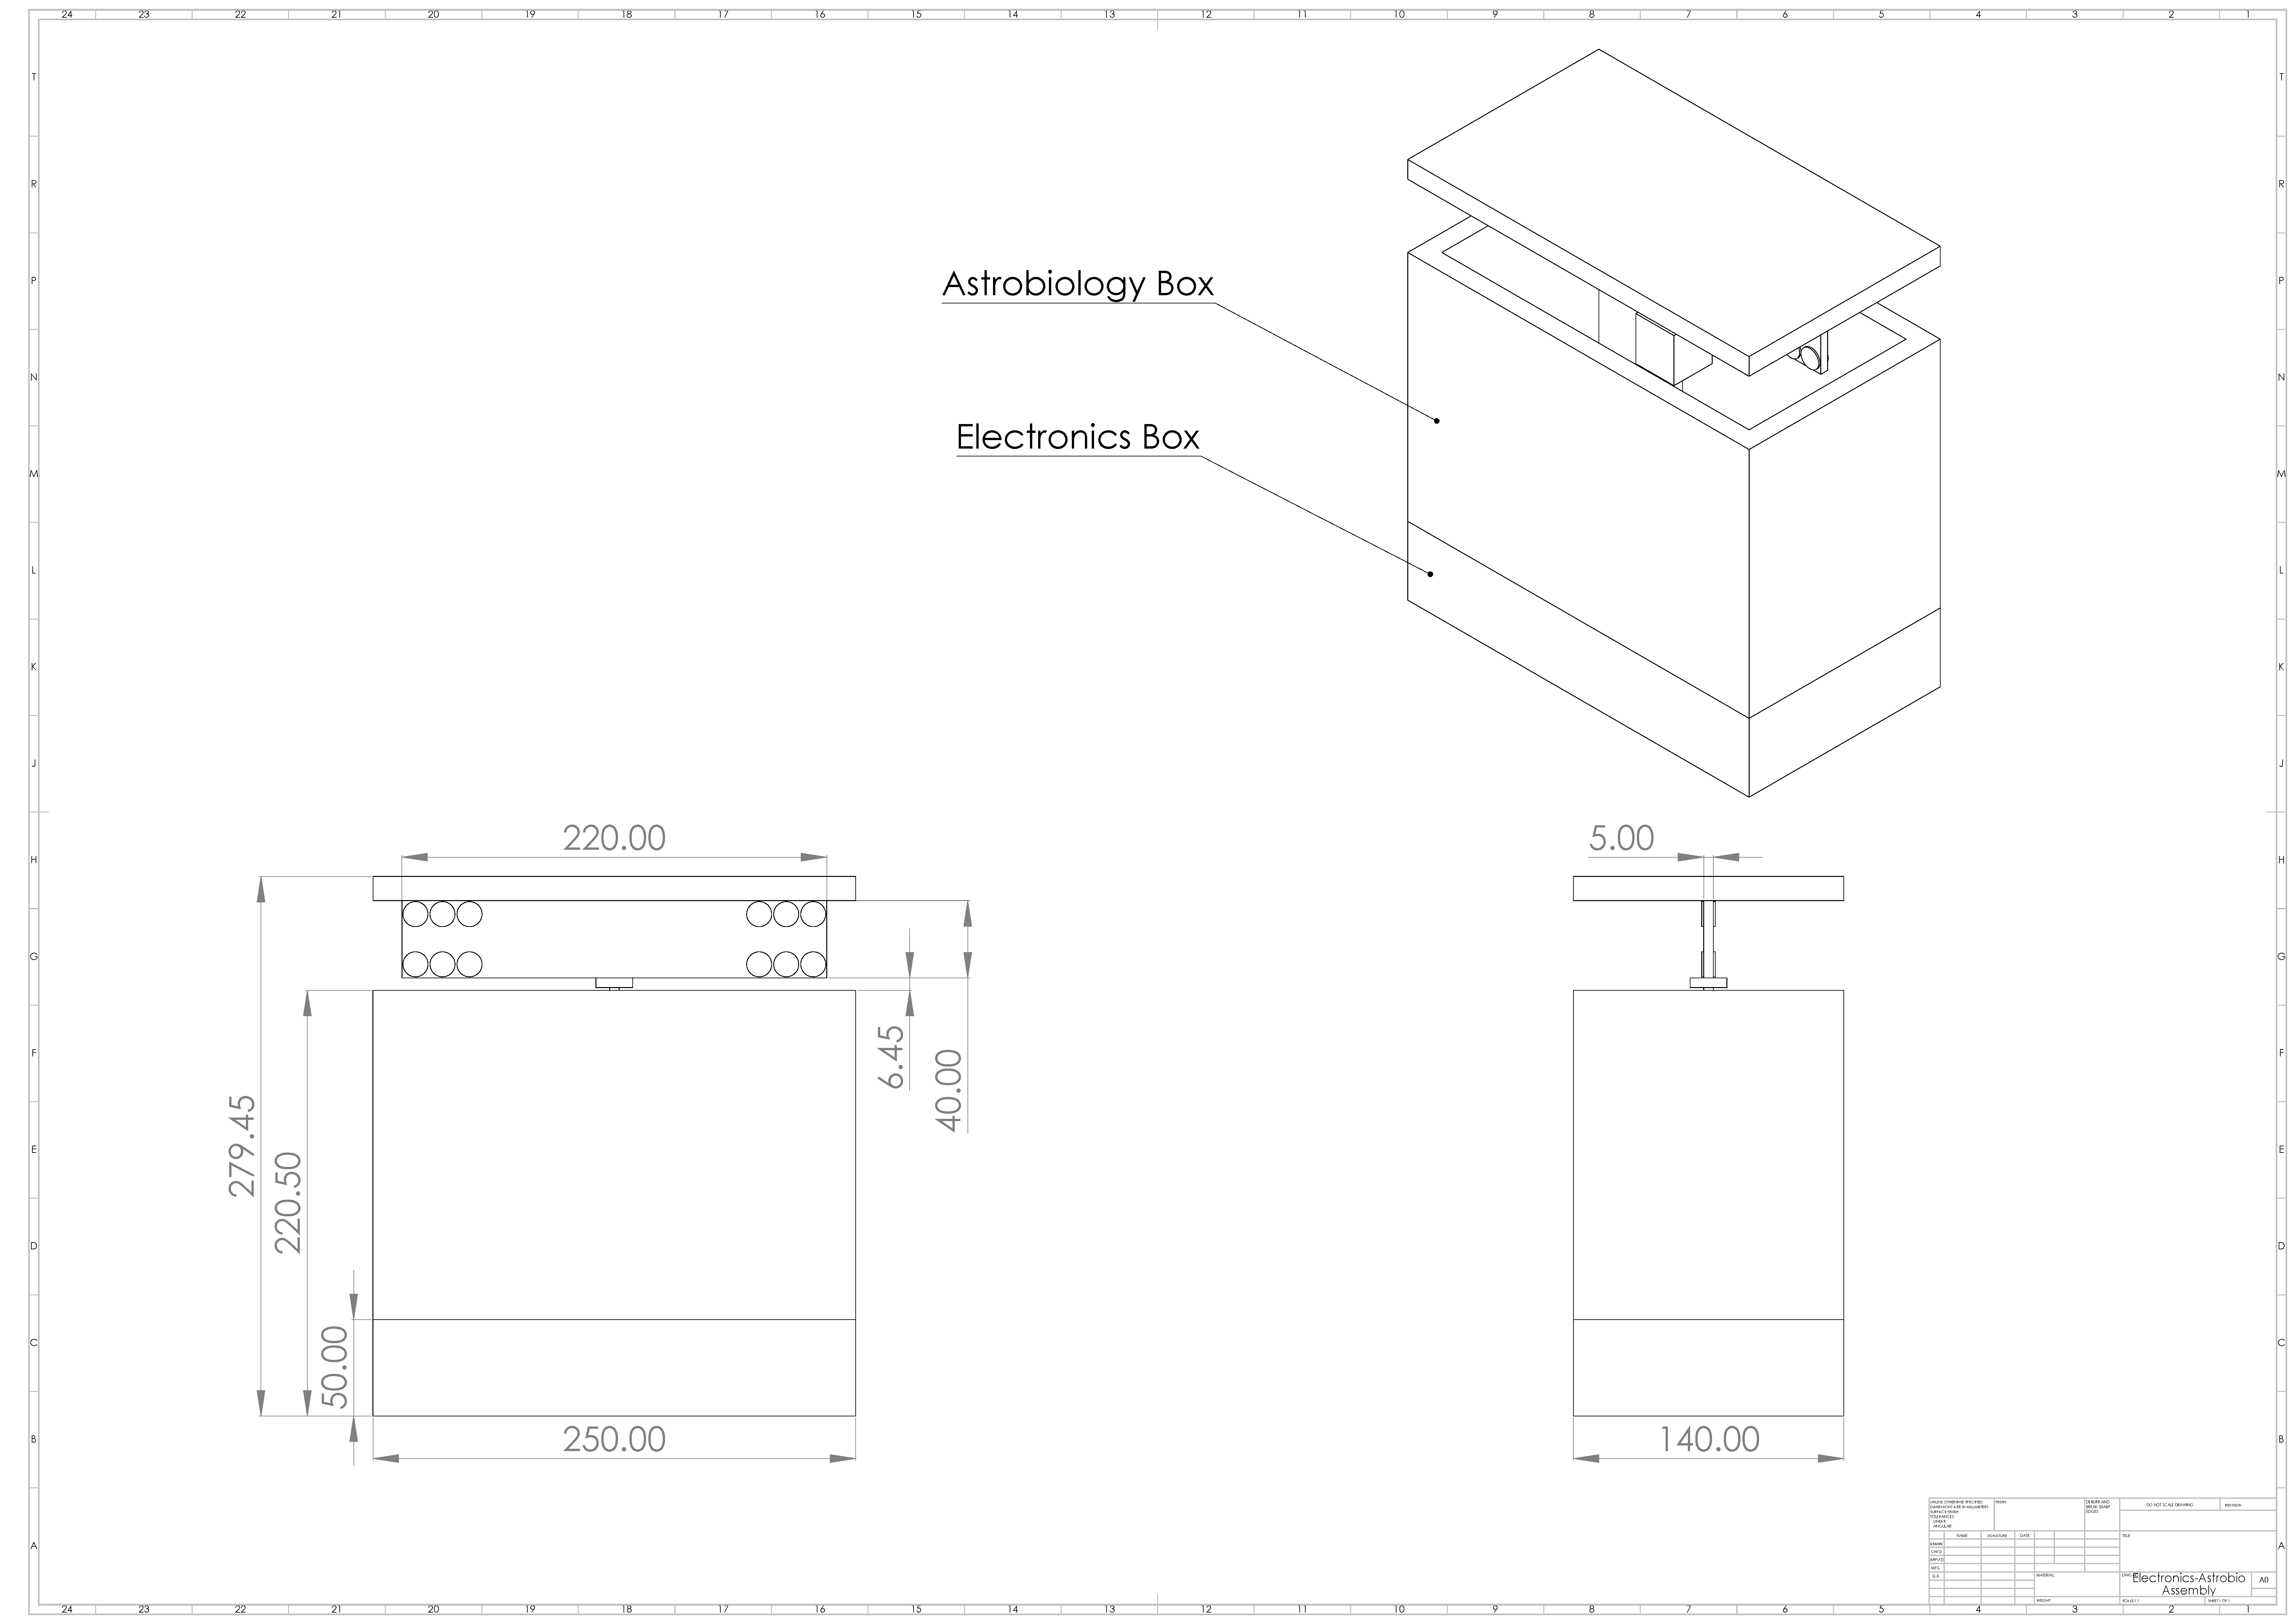
\includegraphics[width=\textwidth]{Figures/astrobio-electronics.pdf}
    \caption{Drawing of the deployed astrobiology system.}
    \label{fig:astrobio-electronics-drawing}
  \end{figure}
  \begin{figure}[h]
    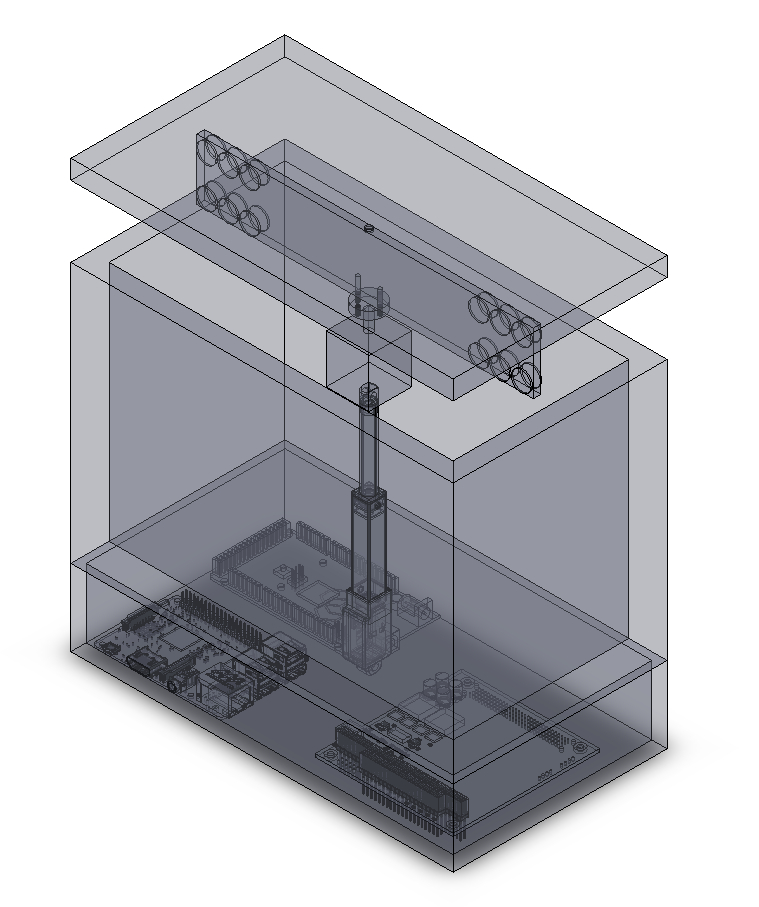
\includegraphics[width=\textwidth]{Figures/astrobio-electronics-deployed-transparent.jpg}
    \caption{Isometric, transparent view of the deployed astrobiology and electronics systems. All electronic components can be seen inside.}
    \label{fig:astrobio-electronics-image}
  \end{figure}
  \begin{figure}[h]
    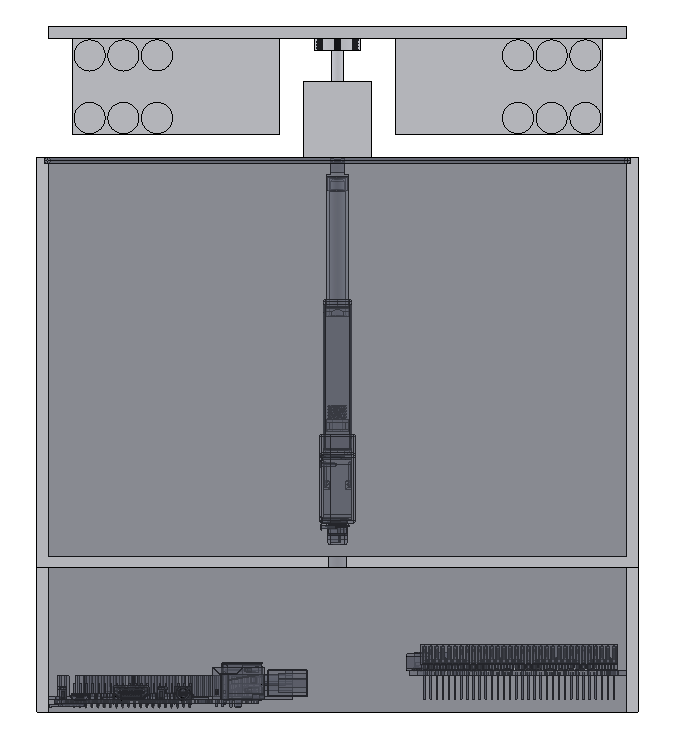
\includegraphics[width=\textwidth]{Figures/astrobio-electronics-deployed-transparent-sideview.png}
    \caption{Transparent Side view of the astrobiology and electronics box.}
    \label{fig:astrobio-electronics-image-sideview}
  \end{figure}

  % ISS system
  \begin{figure}[h]
    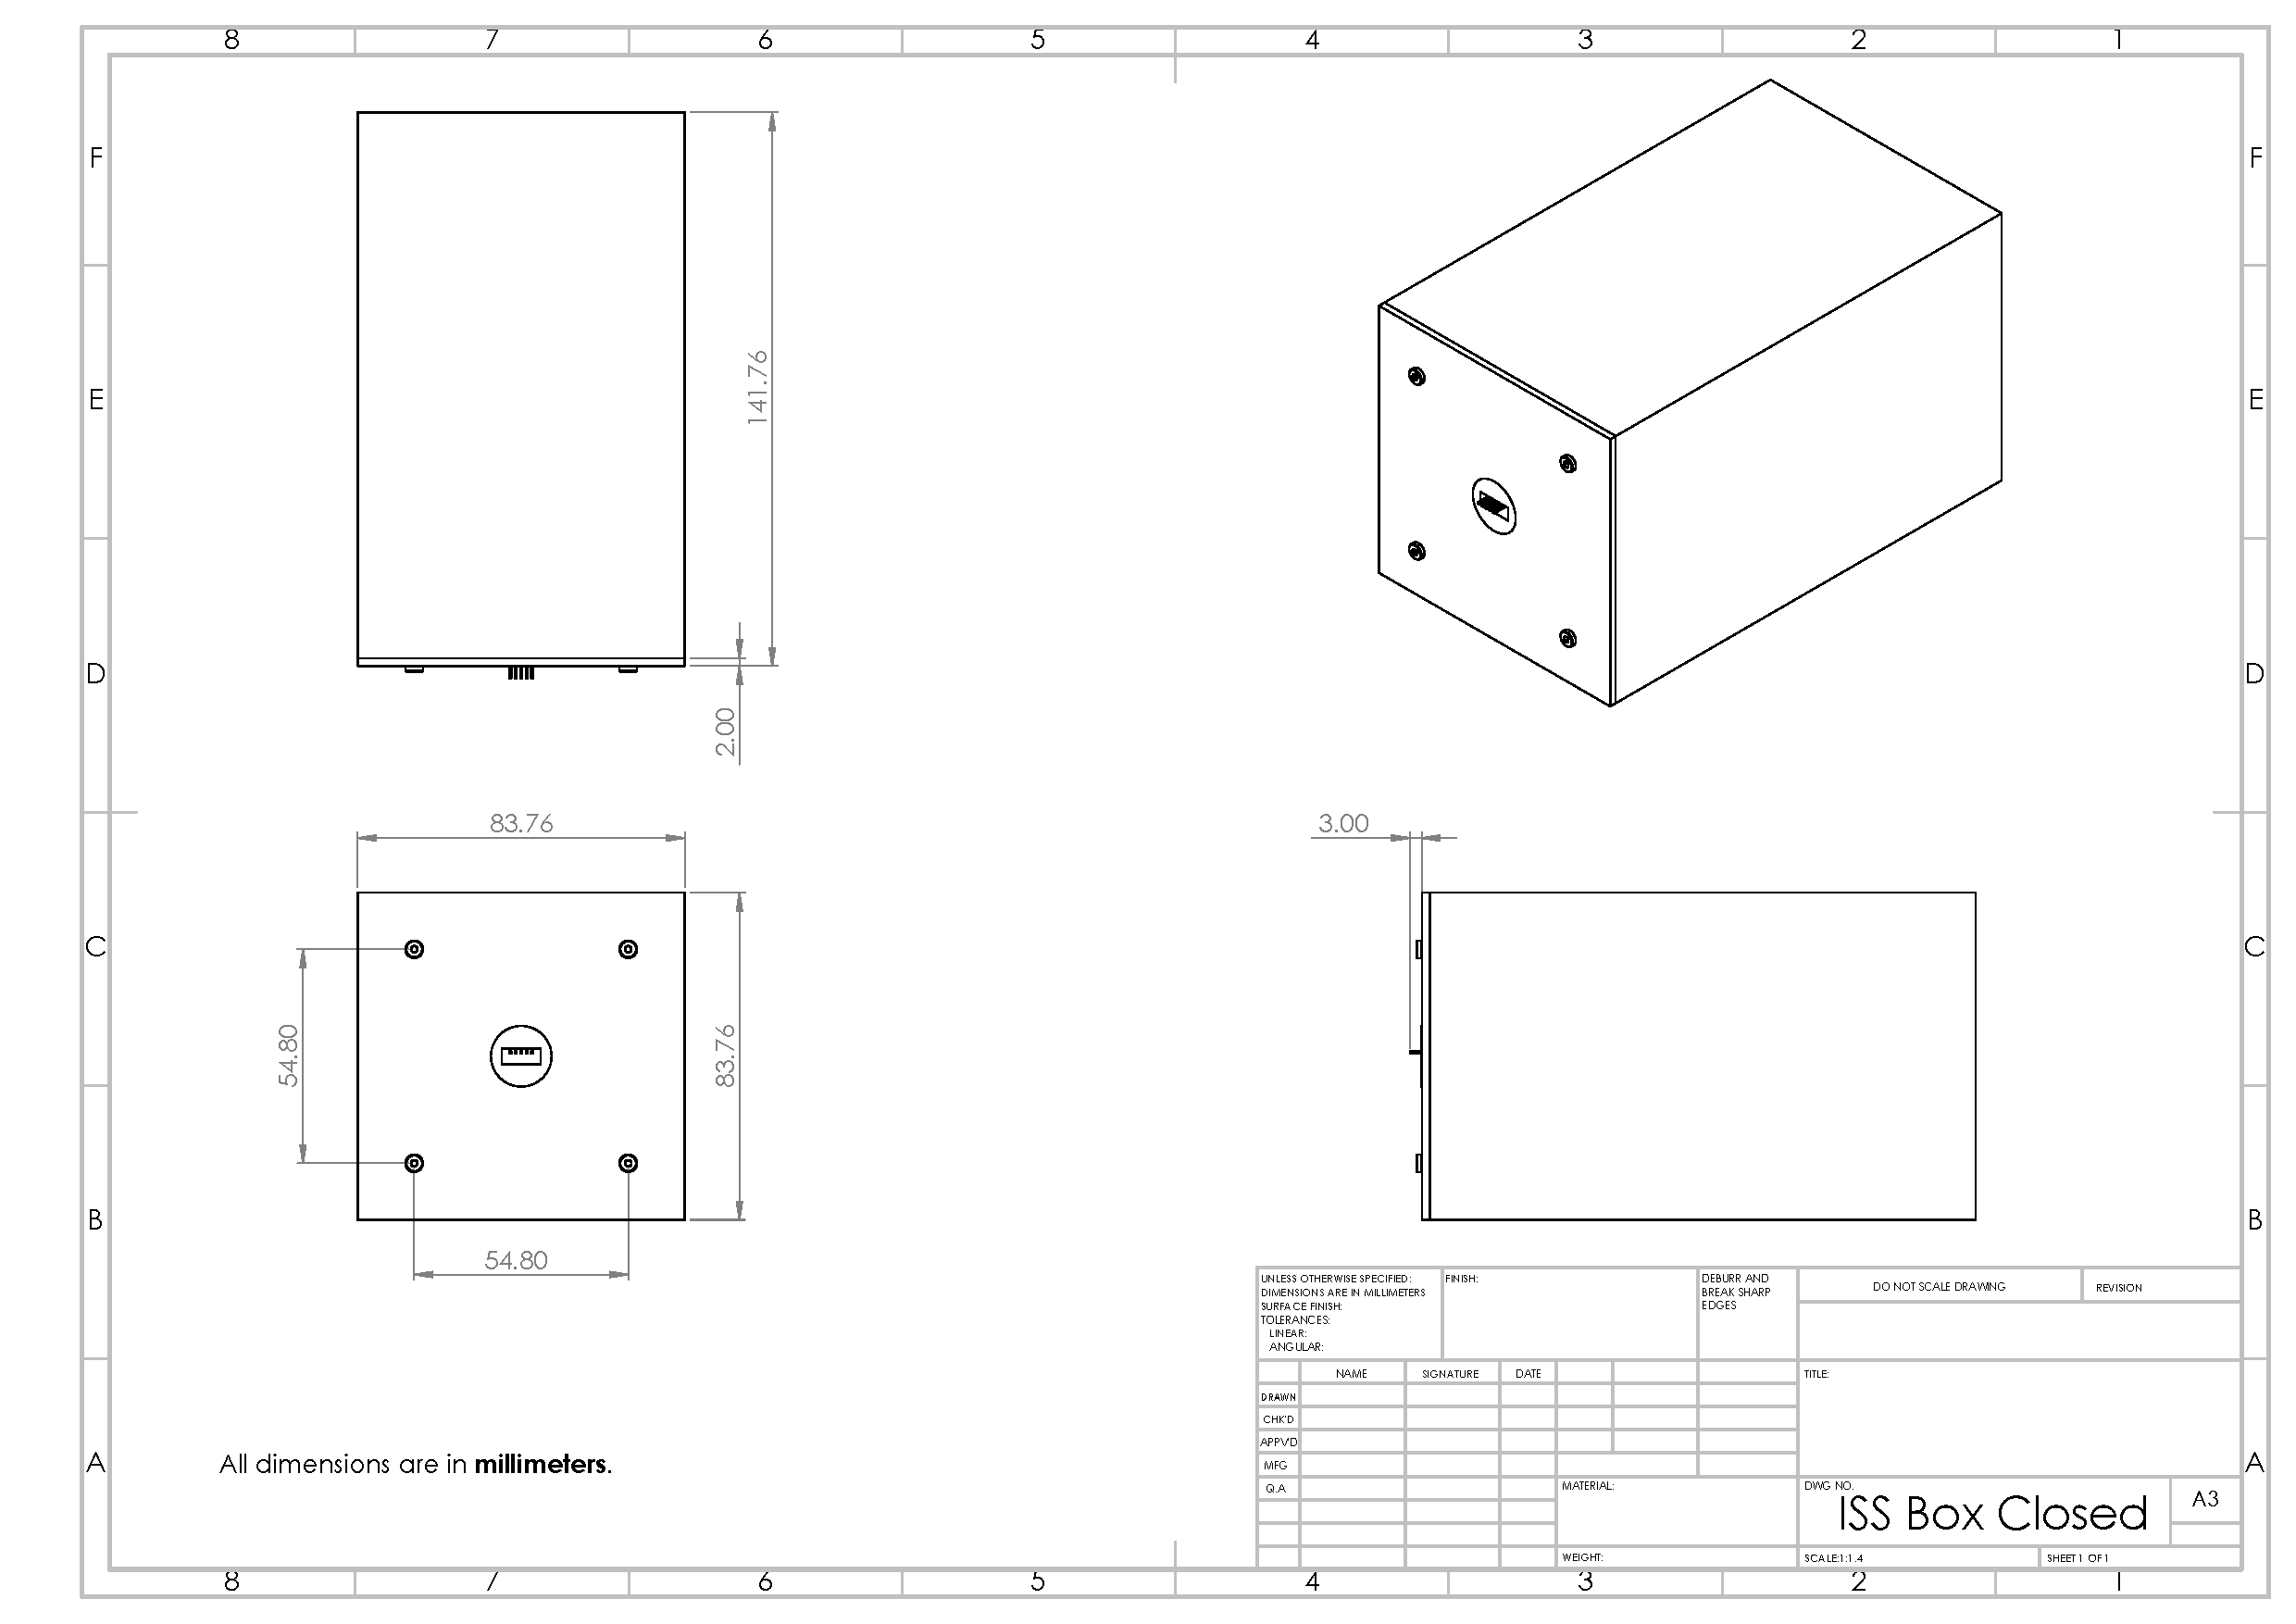
\includegraphics[width=\textwidth]{Figures/iss-closed.pdf}
    \caption{Drawing of the closed ISS module.}
    \label{fig:iss-closed-drawing}
  \end{figure}
  \begin{figure}[h]
    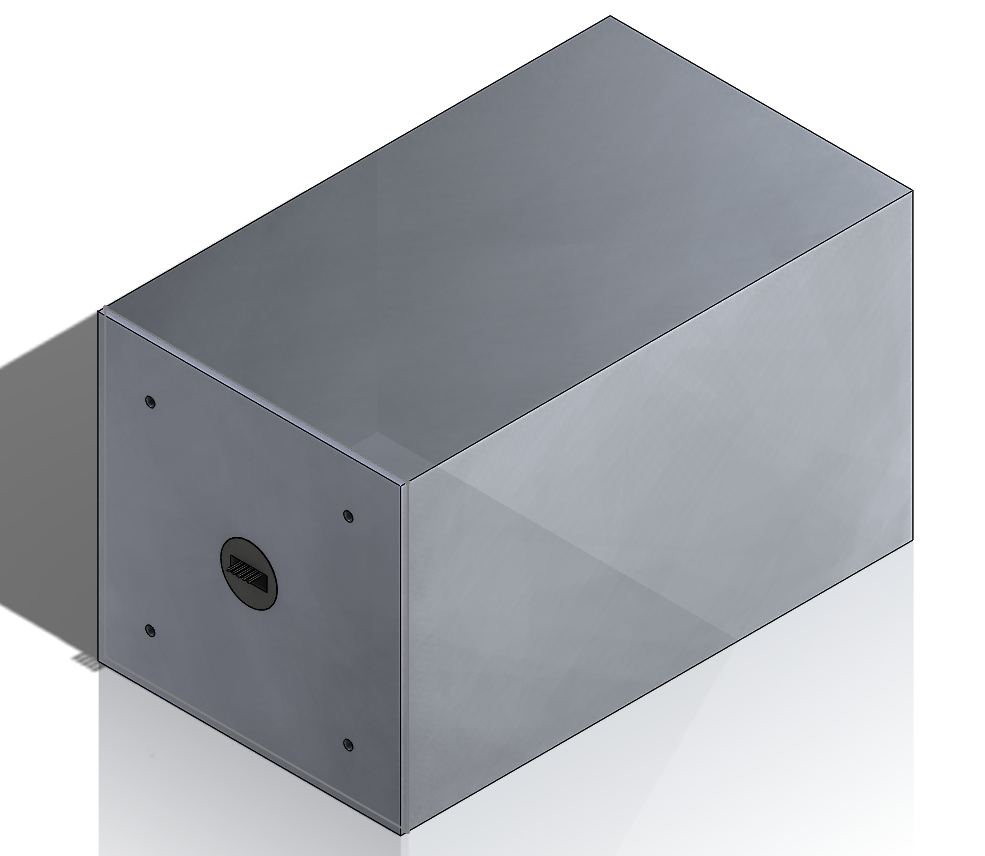
\includegraphics[width=\textwidth]{Figures/iss-closed.png}
    \caption{Isometric view of the closed ISS module.}
    \label{fig:}
  \end{figure}
  \begin{figure}[h]
    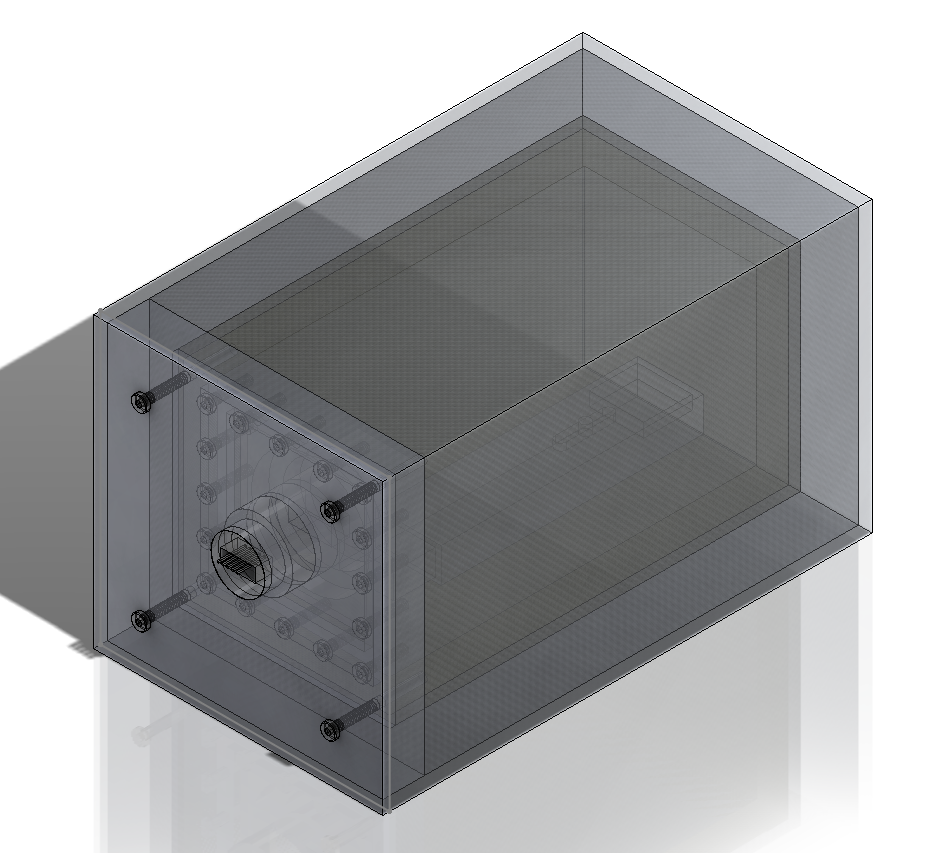
\includegraphics[width=\textwidth]{Figures/iss-closed-transparent.png}
    \caption{Isometric, transparent view of the closed ISS module.}
    \label{fig:iss-closed-transparent-image}
  \end{figure}
  \begin{figure}[h]
    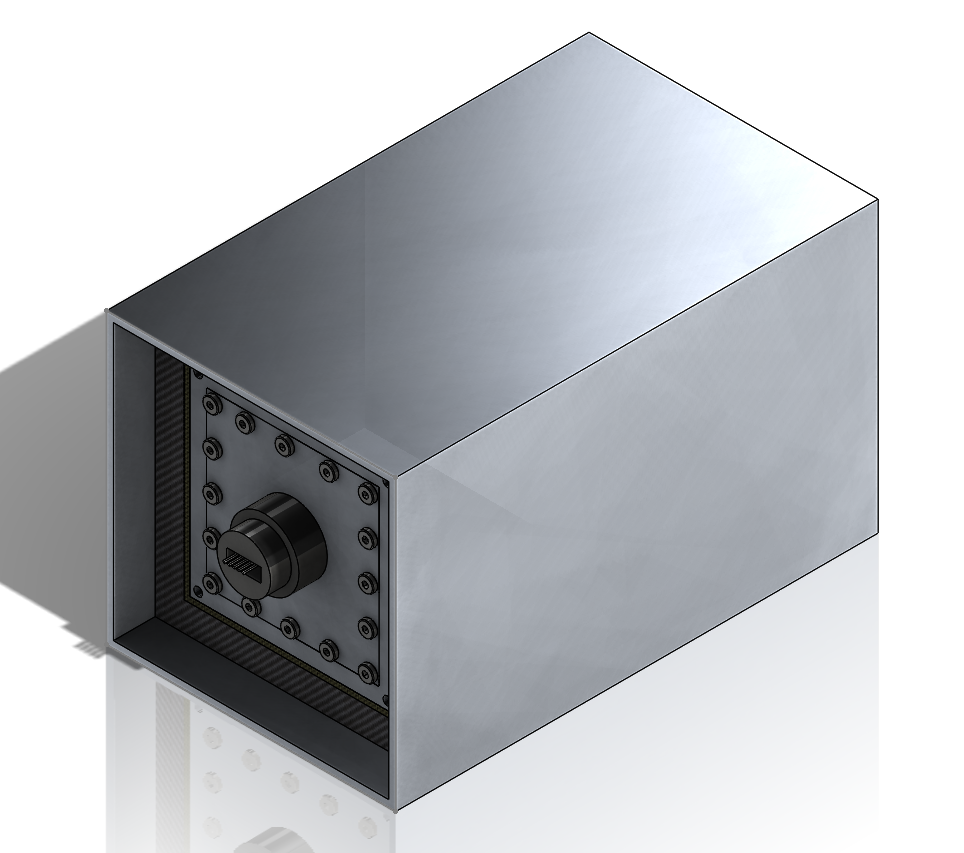
\includegraphics[width=\textwidth]{Figures/iss.png}
    \caption{Isometric view of the ISS showing the casing of the pressurized inner container.}
    \label{fig:iss-image}
  \end{figure}
  \begin{figure}[h]
    %\includegraphics[width=\textwidth]{Figures/}
    \caption{}
    \label{fig:}
  \end{figure}  
  \begin{figure}[h]
    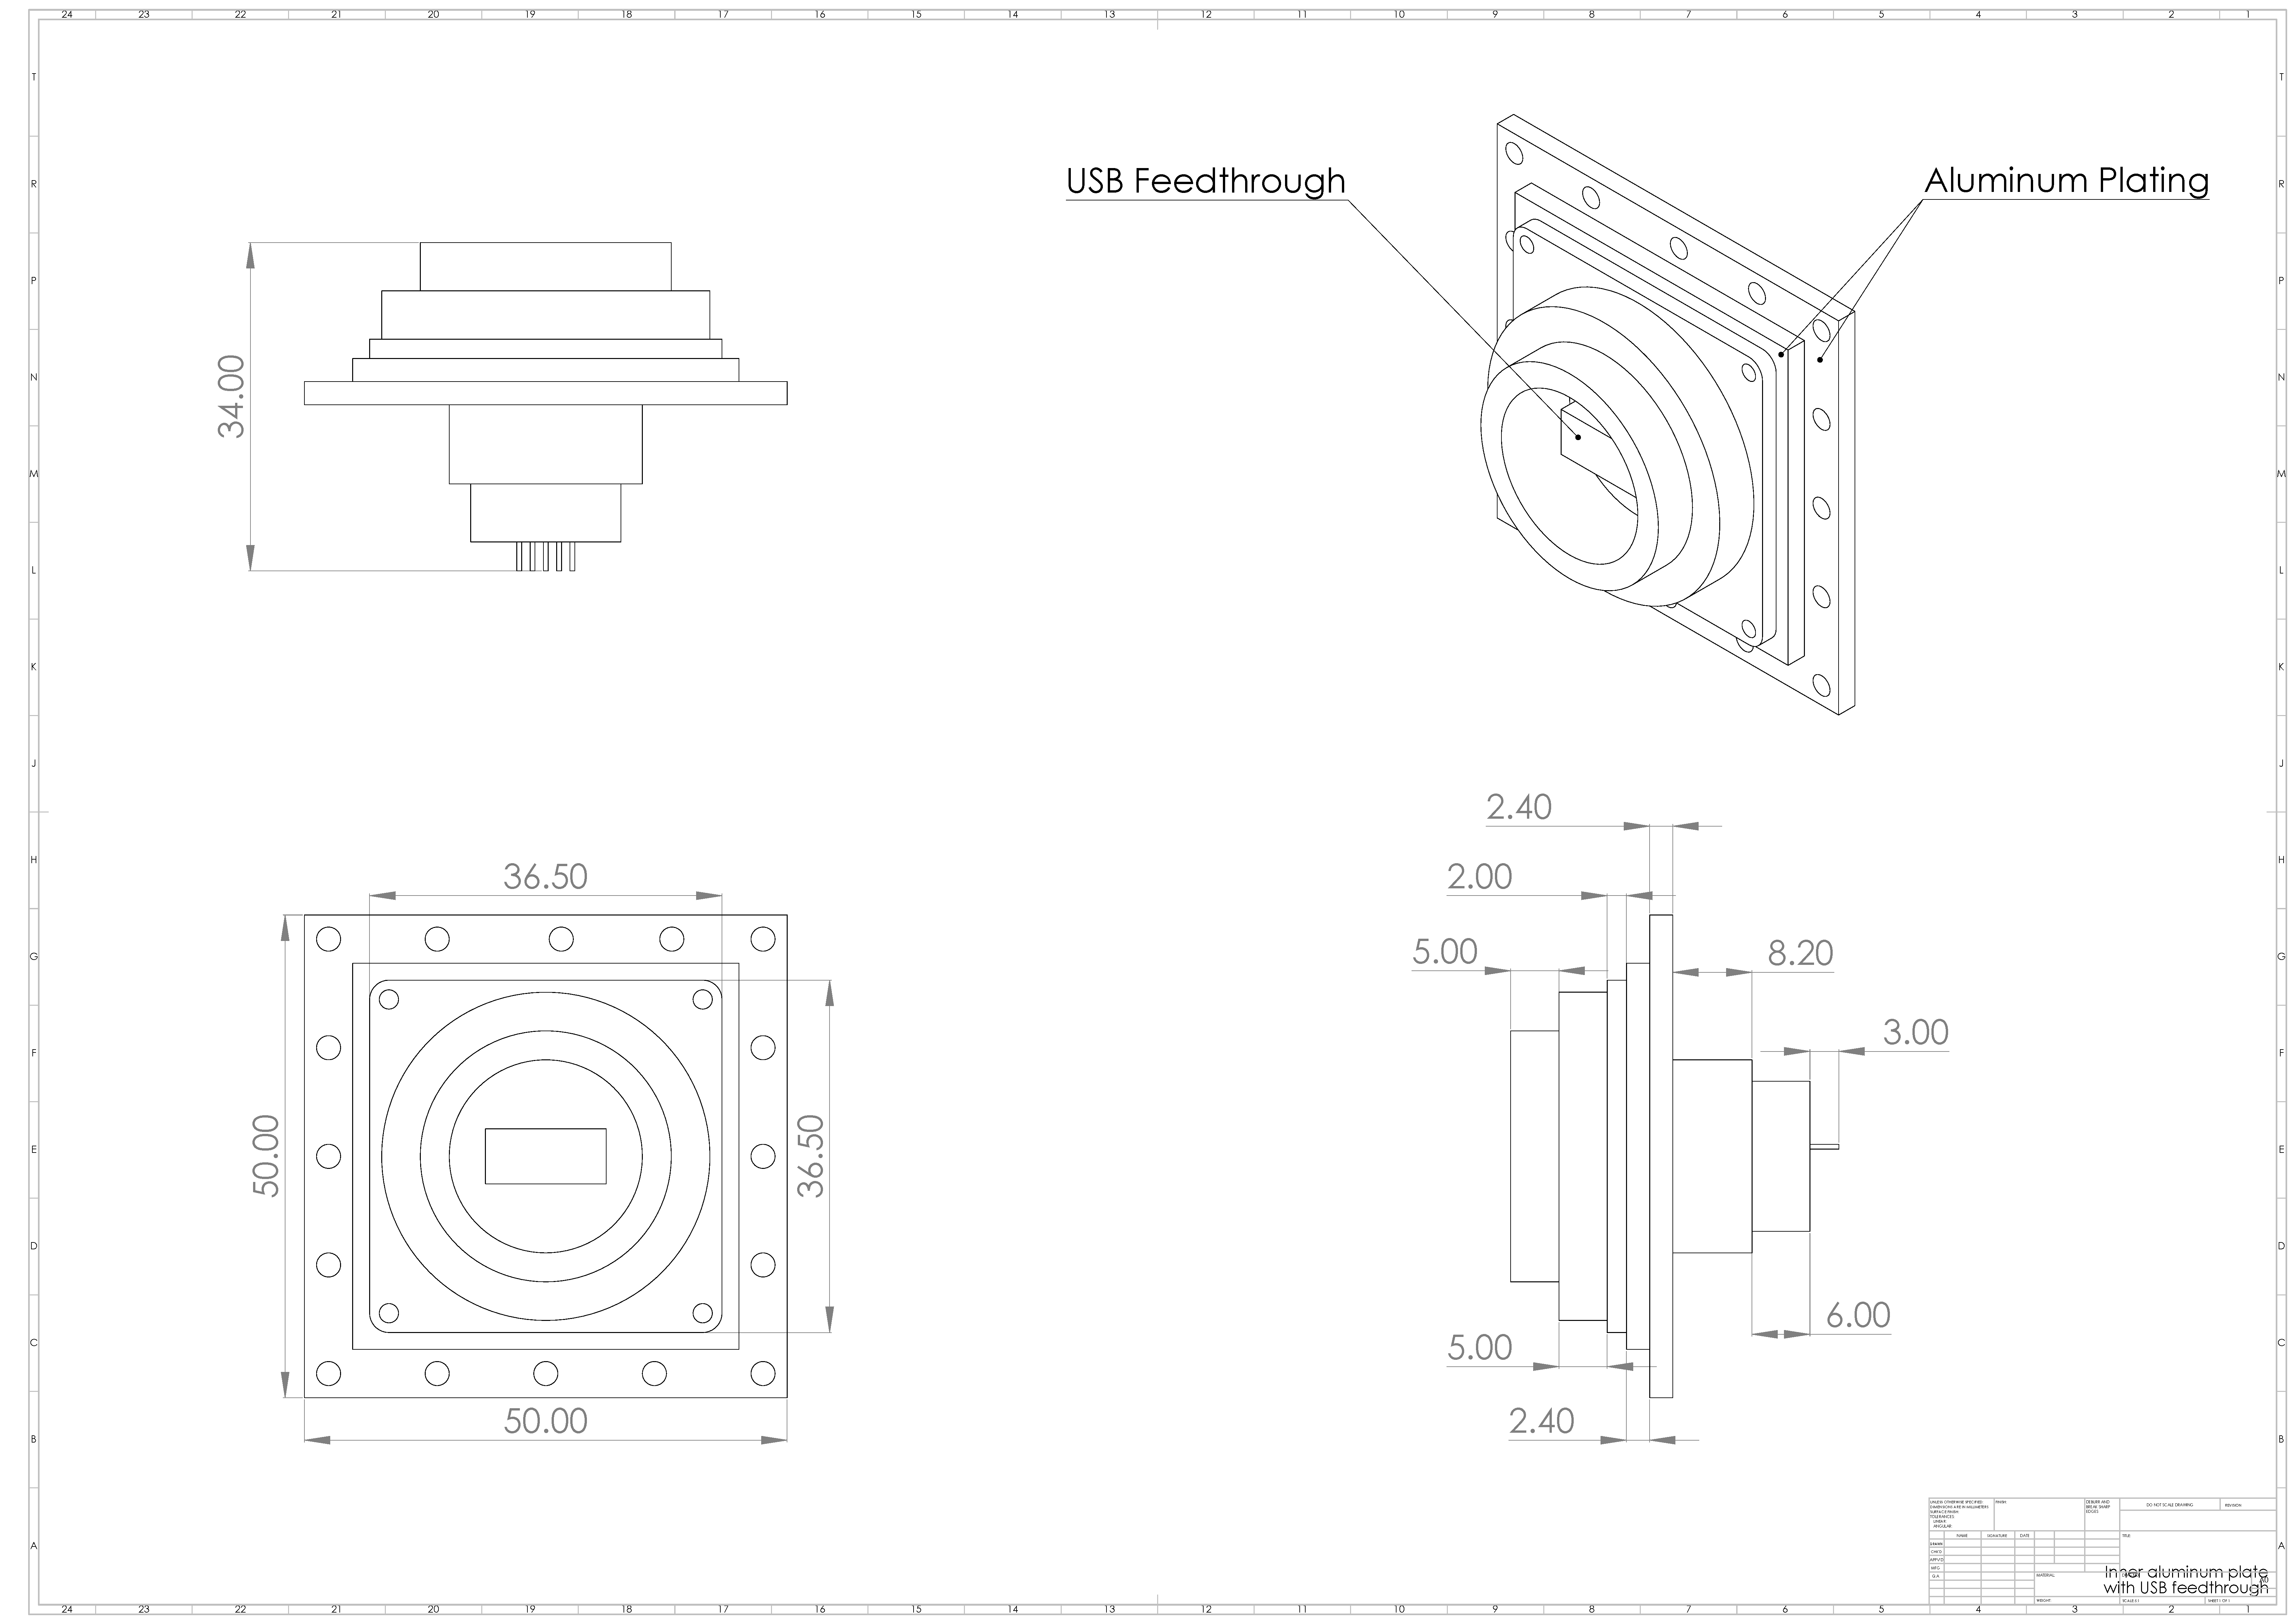
\includegraphics[width=\textwidth]{Figures/inner-aluminum-plate-with-feedthrough.pdf}
    \caption{Removable aluminum plate to contain the atmosphere within the ISS module.}
    \label{fig:InnerAluminumPlate}
  \end{figure}
\end{centering}
